
\pagebreak

\section*{Introduction}
\addcontentsline{toc}{section}{Introduction}
%\markboth{Introduction}{} 
Comme TV5 monde en 2015, les pertes des entreprises victimes de cyberattaques, en forte augmentation, se comptent souvent en dizaines de millions d'euros. L'Open Web Application Security Project (OWASP : {\color{blue} \url{https://www.owasp.org}}), publie régulièrement la liste des 10 menaces les plus critiques qui concernent les applications web. Une manière de s'en prémunir consiste à pratiquer le hacking web éthique. C'est là qu'entre en scène l'outil DVWA. Damn Vulnerable Web App ({\color{blue} \url{http://www.dvwa.co.uk}}), est un environnement PHP qui permet de se former à la sécurité des sites web. Le hacker en herbe peut ainsi se former et tester légalement ses compétences sur une application hébergée en local. Une solution simple consiste à installer la distribution kali et le site web DVWA sur une machine virtuelle.

\begin{figure}[!h]
	\begin{center}
		\label{10_menaces}
		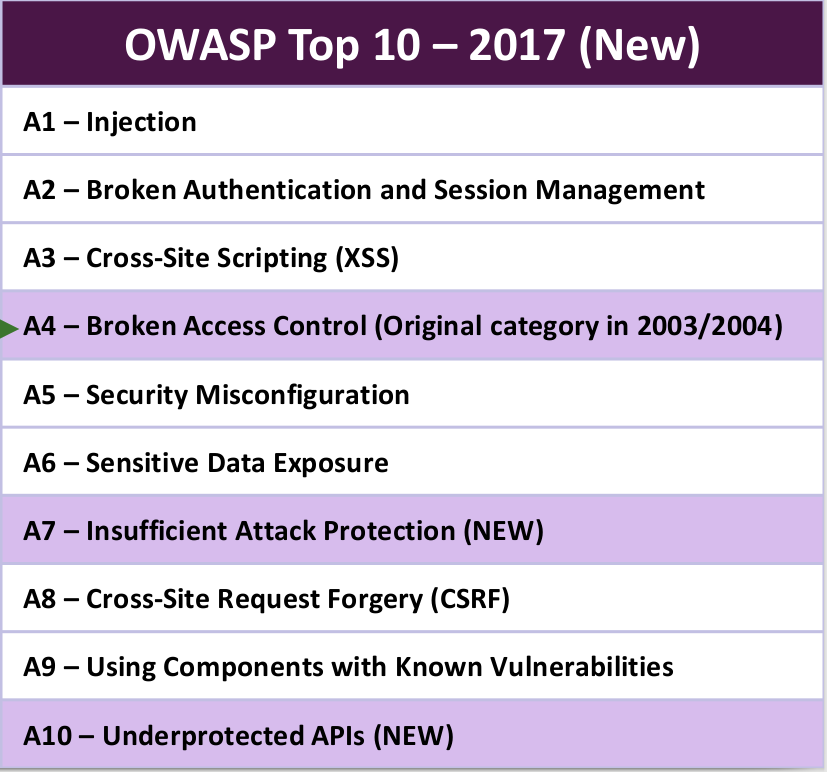
\includegraphics[scale=0.4]{images/10_menaces.png}
		\caption{Le top 10 des menaces web 2017 publiées par l'OWASP}
	\end{center}
\end{figure}



, 
Pour se former au hacking et donc à la sécurité des applications web, 
